\subsection{Hypothesis on Relation Properties}
\label{sec:hypothesis_relation_properties}

This hypothesis is inspired by the fact that some embedding methods are unable to handle specific properties.

\begin{figure*}[htb]
\centering
\begin{minipage}{0.95\textwidth}
\centering
\small
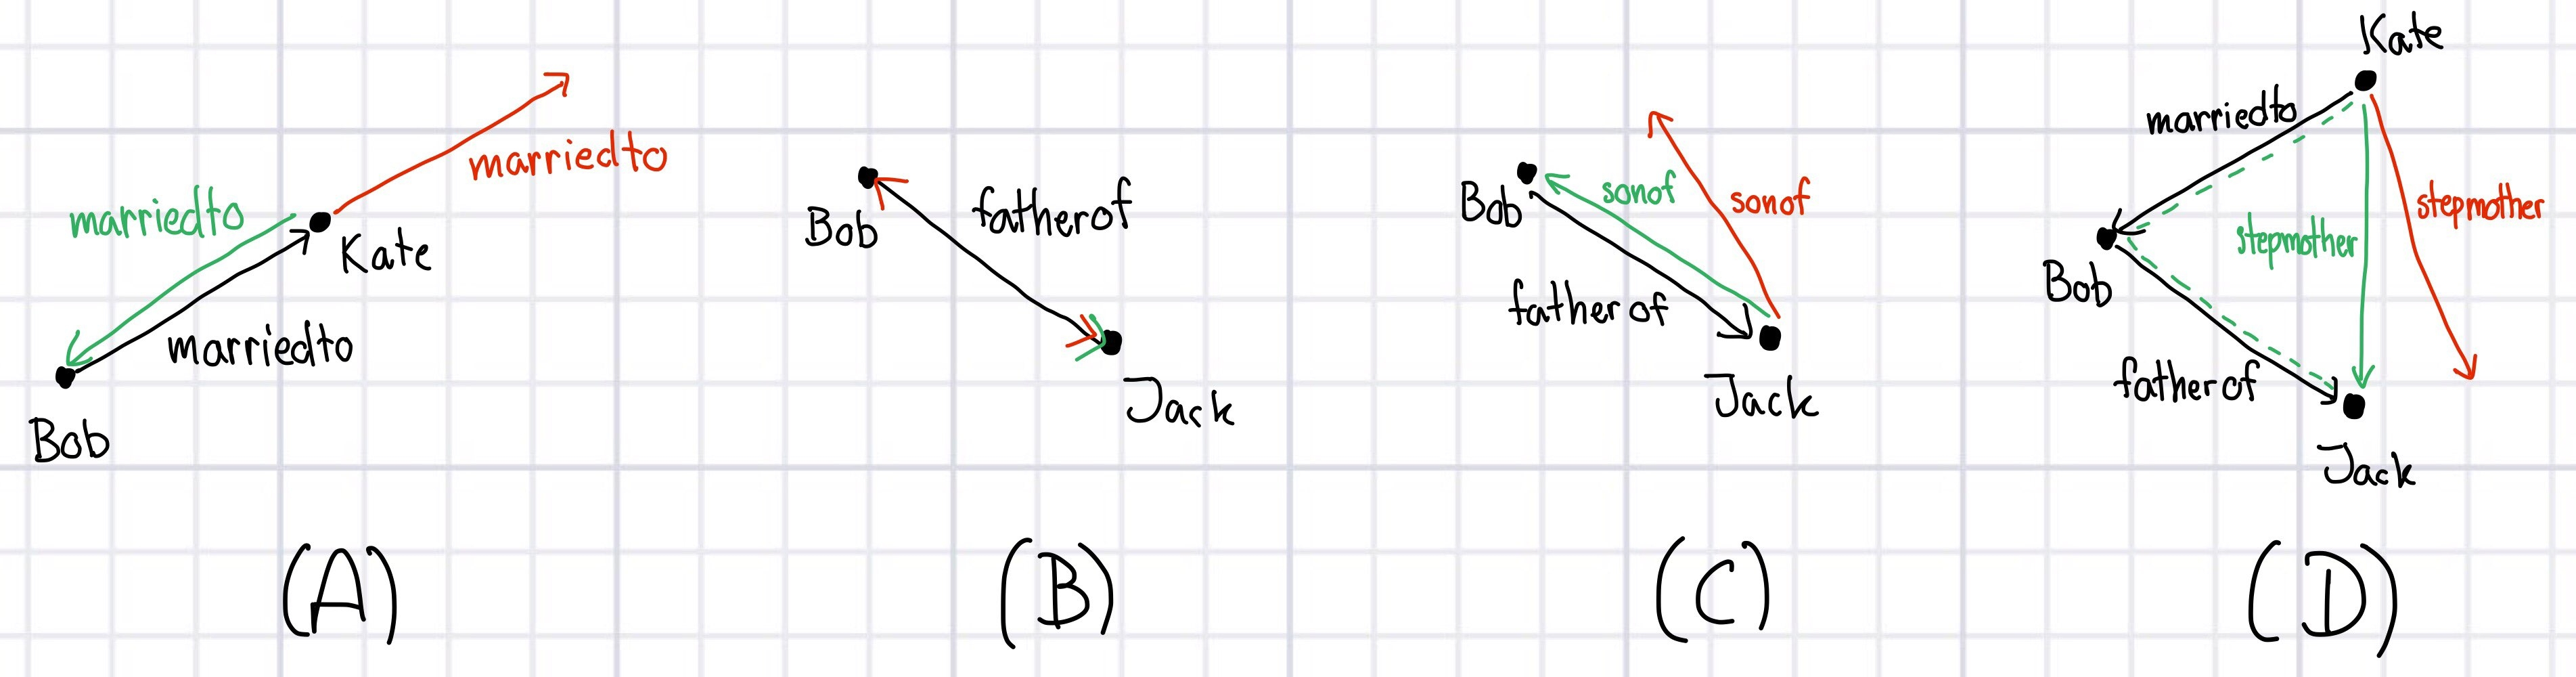
\includegraphics[scale=0.12]{content/hypotheses/figures/relation_properties_A-D.jpg}
\caption{Illustration of \autoref{hyp:relation_properties} A-D. Black is embedded information and red/green are different versions of the same relation embedding. Green is what the embedding should look like if the method can model relations with that property and red is what the embedding might look like if not. A: Symmetry, B: Anti-Symmtery, C: Inversion, D: Composition.
}
\label{fig:relation_properties_nothierarchy}
\end{minipage}
\end{figure*}

\begin{hypothesis}
\label{hyp:relation_properties}
Prediction quality of queries with certain temporally constrained relation properties is significantly higher on methods, which theoretically can model those properties, than methods which cannot.
\end{hypothesis}

For this hypothesis we compare DE-TransE, DE-DistMult and DE-SimplE as they resemble one another and have varied combinations of relation properties that they can and cannot model.
The relation properties selected for analysis are symmetry, anti-symmetry, and inversion. Reflection, composition and hierarchy were considered but disregarded. 
Reflection was disregarded because all considered methods are capable of modeling it and because we found no relation type with that property in any of the datasets.
Composition was disregarded because composition is made up of multiple facts, it is more affected by incomplete data than the remaining relations.
Hierarchy was disregarded as we were unable to identify a method capable of modeling that relation, which was also temporal.
%håndter også udkommenteret definition på reflexion
This hypothesis is divided into several subhypotheses specific to each relation property:

\begin{subhypothesis}
\label{hyp:relation_property_sym}
DE-TransE has worse performance than DE-DistMult and DE-SimplE on link prediction tasks with \textbf{symmetrical} relations.
\end{subhypothesis}

As TransE is a straightforward translational method in Euclidian space, it is incapable of modelling symmetry \cite{goel19diachronicemb}. Theoretically, DE-TransE has the same limitation with temporal symmetrical relations, which are relations that happen simultaniously between two entities. An example of such a relation could be \textit{gets\_married\_to}. The purpose of \autoref{hyp:relation_property_sym} is to empirically analyze the extent of this limitation.

%This subhypothesis is illustrated in \autoref{fig:relation_properties_nothierarchy} A. When Bob is married to Kate, Kate is also married to Bob. If the method cannot model symmetry it may attempt to model Kate's relation to Bob with the same vector it models Bob's relation to Kate. However, in a vector space that would point Kate's relation vector in the opposite direction.

\begin{subhypothesis}
\label{hyp:relation_property_antisym}
DE-DistMult has worse performance than DE-TransE and DE-SimplE on link prediction tasks with \textbf{anti-symmetrical} relations.
\end{subhypothesis}

DistMult uses pairwise interactions in diagonal matrices, and as such cannot model edge direction, which in turn means it cannot model anti-symmetry \cite{goel19diachronicemb}. Theoretically, DE-DistMult has the same problem, but for temporal anti-symmetrical relations, which are relations where an entity performs an action to another entity and that other entity cannot do the same action back in the same timespan. An example of such a relation is \textit{arrest}, as this is something a police force does to citizens, but citizens cannot do to a police force. The purpose of \autoref{hyp:relation_property_antisym} is to empirically analyze the extent of this limitation.

%This hypothesis is illustrated in \autoref{fig:relation_properties_nothierarchy} B. When Bob is the father of Jack, Jack cannot be the father of Bob. If the method cannot model anti-symmetry it may not know the direction of the vector and as such it does not know who is the father of whom.

\begin{subhypothesis}
\label{hyp:relation_property_inv}
DE-DistMult has worse performance than DE-TransE and DE-SimplE on link prediction tasks with \textbf{inverse} relations.
\end{subhypothesis}

As DistMult cannot model edge direction, it also cannot model inversion \cite{goel19diachronicemb}. Theoretically, DE-DistMult has the same problem, but for temporal inverse relations, which are pairs of relation types, where when one entity relates to another with one type, they are also related in the opposite direction with the other type, both relations happening in the same timespan. An example of such a pair is the relations \textit{host\_a\_visit} and \textit{make\_a\_visit}. The purpose of \autoref{hyp:relation_property_inv} is to empirically analyze the extent of this limitation.

To analyze these subhypotheses, the test sets are divided into sets of facts that contain only relations of that type and sets of facts that contain all but that relation type. The first step is to assign a number of soft labels to each relation type, using a function for each relation property that maps each relation type to a real number $\varR \rightarrow [ 0 , 1 ]$. This function describes how many facts that fulfill the requirements for that relation type. The reasoning for this is that knowledge graphs are not complete, and some relations might be missing from the graph.

The symmetry soft label for relation $r$ is

\begin{equation}
\begin{gathered}
\mathit{sym}(r) = \frac{|S|}{|\eta_r|}\\
S = \{ (e_1, r, e_2, \tau) \in \eta_r \mid (e_2, r, e_1, \tau) \in \eta_r \}
\end{gathered}
\end{equation}

\noindent
The anti-symmetry soft label for relation $r$ is

\begin{equation}
\begin{gathered}
\mathit{asym}(r) = \frac{|A|}{|\eta_r|}\\
A = \{ (e_1, r, e_2, \tau) \in \eta_r \mid (e_2, r, e_1, \tau) \notin \eta_r \}
\end{gathered}
\end{equation}

\noindent
The inversion soft label for relation $r$ is

\begin{equation}
\begin{gathered}
\mathit{inv}(r) = \varmax_{r^i \in \varR \setminus \{r\} } \frac{|I_{r^i}|}{|\eta_{r^i}|}\\
I_{r^i} = \{ (e_2, r^i, e_1, \tau) \in \eta_{r^i}  \mid (e_1, r, e_2, \tau) \in \eta_r \}
\end{gathered}
\end{equation}

% \noindent
% The reflexivity soft label for relation $r$ is

% \begin{equation}
% \begin{gathered}
% \mathit{ref}(r) = \frac{|R|}{|\eta_r|}\\
% R = \{ (e_1, r, e_2, \tau) \in \eta_r \mid e_1 = e_2 \}
% \end{gathered}
% \end{equation}

We define a threshold for each of these relation properties, and classify each relation type as being symmetrical, anti-symmetrical, and/or inverse, if the soft label for that relation type is higher than or equal to the threshold. Any relation type can be classified with any number of relation properties. The threshold for symmetry is $0.8$, for anti-symmetry is $1.0$, and for inverse is $0.8$.
%and for reflexivity is $0.8$.
The set of facts where the relation is symmetrical ($T_S$), as well as the set of test facts where the relation is not symmetrical ($T_S'$), on testset $T$ is defined

\begin{equation}
\begin{aligned}
T_S & = \{ (h, r, t, \tau) \in T \mid \mathit{sym}(r) \geq 0.8 \}\\
T_S' & = \{ (h, r, t, \tau) \in T \mid \mathit{sym}(r) < 0.8 \}
\end{aligned}
\end{equation}

\noindent
Similarly, the anti-symmetric test facts $T_A$, the not anti-symmetric test facts $T_A'$, the inverse test facts $T_I$, and the non-inverse test facts $T_I'$ are defined, using their respective thresholds.

The models are evaluated over these property specific test sets for each dataset and compared to one another. 
We expect the models that theoretically are able to express a relation property to have similar scores on the test sets with and without the property represented.
Conversely, we expect the models that are not to have a significantly lower score on the test set where the property is represented than the one where it is not.
If this is the case the hypothesis is deemed true.